\documentclass[twocolumn]{aastex61}

\usepackage[utf8]{inputenc}
\usepackage{xspace}
\usepackage{url}
\usepackage{listings}
\usepackage{inconsolata} % standard "prettier" astropy latex font

\usepackage{listings}

\newcommand{\package}[1]{\texttt{#1}\xspace}
\newcommand{\astroquery}{\package{astroquery}}
\newcommand{\astropy}{Astropy\xspace}
\newcommand{\astropypkg}{\package{astropy}}

\definecolor{dkgreen}{rgb}{0,0.6,0}
\definecolor{gray}{rgb}{0.5,0.5,0.5}
\definecolor{mauve}{rgb}{0.58,0,0.82}

\renewcommand{\lstlistingname}{Example}
\lstset{frame=tb,
  language=Python,
  aboveskip=3mm,
  belowskip=3mm,
  showstringspaces=false,
  columns=flexible,
  basicstyle={\small\ttfamily},
  numbers=none,
  numberstyle=\tiny\color{gray},
  keywordstyle=\color{blue},
  commentstyle=\color{dkgreen},
  stringstyle=\color{mauve},
  breaklines=true,
  breakatwhitespace=true,
  tabsize=3,
}

\begin{document}
\newcommand{\nraojansky}{\affiliation{\it{Jansky fellow of the National Radio Astronomy Observatory, 1003 Lopezville Rd, Socorro, NM 87801 USA }}}

\author[0000-0001-6431-9633]{Adam Ginsburg}
\nraojansky

\correspondingauthor{Adam Ginsburg}
\email{aginsbur@nrao.edu; adam.g.ginsburg@gmail.com}

\author{Brigitta Sipocz}

\author[0000-0003-2528-3409]{Brett M. Morris}
\affiliation{Astronomy Department, University of Washington, Seattle, WA 98195, USA}

\author[0000-0002-8642-1329]{Thomas P. Robitaille}
\affiliation{Aperio Software Ltd., Headingley Enterprise and Arts Centre, Bennett Road, Leeds, LS6 3HN, United Kingdom}

\author[0000-0001-9898-5597]{Leo P. Singer}
\affiliation{Astroparticle Physics Laboratory, NASA Goddard Space Flight Center, Mail Code 661, Greenbelt, MD 20771, USA}
\affiliation{Joint Space-Science Institute, University of Maryland, College Park, MD 20742, USA}

\author{the Astroquery collaboration, a subset of the astropy collaboration}


\title{\astroquery: An Astronomical Web-Querying Package in Python}

\begin{abstract}
\astroquery is a collection of tools for requesting data from databases hosted
on the internet, particularly those with web pages but without formal
application program interfaces (APIs).  These tools are based on the Python
\package{requests} package, which is used to make HTTP requests, and
\astropypkg, which provides most of the data parsing functionality. \astroquery
has received significant contributions from the broader astronomical community,
including several significant contributions from telescope archives.
\astroquery enables the creation of fully reproducible workflows from data
acquisition through publication.  This document describes the philosophy, basic
structure, and development model of the \astroquery package.
\footnote{
The repository associated with this paper is:
https://github.com/adamginsburg/astroquery-paper
}
\end{abstract}


\section{Introduction}
Sharing data is a critical component of astronomical research.  Astronomy
has historically been a leading field in data sharing, motivated at least
in part by questions that cannot be answered with single instruments.
In the past few decades, blind surveys have played a huge role in advancing our
understanding of the universe, and these surveys have produced large reservoirs
of data that astronomers regularly access.  However, tools for accessing these
reservoirs are heterogeneous and often only available via graphical user
interfaces (GUIs) such as web sites.

One of the cornerstones of research is reproducibility. To be able to reproduce
research, the data need to be available to everyone. Many scientific journals
encourage or demand that the underlying data  accompany the article or be
uploaded to a hosting service. Data sharing is not only important for new
results, but also to provide the ability to test and verify published results.
While many different efforts to promote data sharing have made it more
common, it is difficult to keep track of how and where to retrieve a given data
set. A common scripted interface to tie all these services together is a good
way to make all the different data more accessible, and it provides authors
with the ability to make the full analysis process they used - from data
download to publication - repeatable.

Data sharing has taken on a variety of forms.  The most prominent are the major
observatory archives: MAST, NOAO, ESO, IPAC, CADC, CDS (hosting Vizier and
SIMBAD), NRAO, CXC, HEASARC, and ESA are the main
organizations hosting raw and processed data from ground and space based
telescopes.  These data archives also serve as the primary means for serving data
to users when the data are taken in queue mode, i.e., when the data are taken
while the observer is not on-site.

In addition to observatories and telescopes, individual surveys often share
their full data sets.  In some cases, these data sets are shared via the
observatory that acquired them, for example, the all-sky data acquired with
Planck, WMAP, and COBE.  Other surveys, particularly ground-based surveys,
serve their own data.  Examples include SDSS, 2MASS, UKIDSS, and likely many
more in the near future.

Individual teams and small groups will often share their data.
These services do not follow any particular standard and can be widely
varied in the type and amount of data shared.  Sometimes these data
are shared via the archive systems (e.g., IRSA at IPAC hosts many
individual survey data sets), while others use their own web hosting
systems (e.g., MAGPIS).

Finally, there are other data types relevant to astronomy that are not
served by the typical astronomical databases.  Examples include databases of
molecular and atomic properties, such as those provided by Splatalogue and
NIST, or services that are computationally intensive or require constant
updates, like Solar System ephemerides.  

\astroquery arose from a desire to access these databases from the command line
in a scriptable fashion.  Script-based data access provides astronomers with
the ability to make reproducible analysis scripts in which the data are
acquired and processed into scientifically relevant results with minimal
overhead.

In this paper, we provide an overview of the \astroquery package.
Section \ref{sec:software} describes the basic layout of the software and
the shared API concept underlying all modules.  Section \ref{sec:development}
describes the development model.

% The Virtual Observatory has some overlap with astroquery, but it does not
% provide the simple tools many astronomers find necessary in day-to-day work.
% Additionally, many of the services noted above do not support VO standards or
% protocols and are therefore inaccessible to the VO.


\section{The Software}
\label{sec:software}
\astroquery consists of a collection of modules that mostly share a similar
interface, but are meant to be used independently.  They are primarily based on
a common framework that uses the Python \package{requests} package to perform
HTTP requests to communicate with web services.

For new development, there is a \texttt{template}  that lays out the basic
framework of any new module.  All modules have a single core
\texttt{class} that has some number of associated \texttt{query\_*} methods.
The most common query methods are \texttt{query\_region}, which usually provide
a ``cone search'' functionality, i.e., they search for data within a circularly
symmetric region projected on the sky.

An example using the SIMBAD interface is shown below (see
\url{http://astroquery.readthedocs.io/en/latest/simbad/simbad.html}):
\begin{lstlisting}[caption=Query SIMBAD for a region around M81]
from astroquery.simbad import Simbad
result_table = Simbad.query_region("m81")
\end{lstlisting}
In this example, \texttt{Simbad} is an instance of the
\texttt{astroquery.simbad.SimbadClass} class.
The returned result, stored in the variable \texttt{result\_table},
is an \astropypkg table.

While there is a common suggested API described in the \texttt{template} module,
individual packages are not \emph{required} to support this API because, for
some, it is not possible.  For example, the atomic and molecular databases refer
to physical data that is not related to positions on the sky and therefore
their \astroquery modules cannot include \texttt{query\_region} methods. The same applies to Solar System object ephemerides queries. Differences in the API are discussed in the \astroquery documentation (see Section \ref{sec:documentation}).

\subsection{Version Numbers}
\label{sec:versionnumbers}
\astroquery uses the same format as traditional semantic versioning,
with versions indicated in the format MAJOR.MINOR.PATCH.devCOMMIT\_ID (for
example, 0.3.9.dev4581).  

Starting in mid-2018, \astroquery switched from a manual release model
to a continuous deployment model.  Prior to this change, the MAJOR.MINOR.PATCH
versions were each created manually by one of the maintainers, then pushed
to package release services.  After this change, each accepted pull request
automatically triggered a new release via the python package index
(\url{https://pypi.org/}). 

\astroquery patches are frequently made to accommodate upstream changes, i.e.,
changes made to the remote service, and as such are not guaranteed to be
backward-compatible.

\subsection{HTTP User-Agent}
\label{sec:useragent}
\astroquery identifies itself to host services using the \texttt{HTTP
User-Agent} header data.  The format of the User-Agent string is
\texttt{astroquery/\{version\} \{requests\_version\}}, where
\texttt{\{version\}} is a version number of the form described in \S
\ref{sec:versionnumbers} and \texttt{\{requests\_version\}} is the
corresponding version of the Python
\package{requests} package.  This information can be used by data hosting services
to determine how many users are accessing their service via \astroquery
and to assist in debugging if improper queries are being submitted.


\subsection{The API}
The common API has a few features defined in the \texttt{template} module.
Each service is expected to provide the following interfaces, assuming they are
applicable:

\begin{itemize}
    \item \texttt{query\_region} - A function that accepts an \astropypkg
        \texttt{SkyCoord} object representing a point on the sky plus a
        specification of the radius around which to search.
        The returned object is an \astropypkg \texttt{Table}.
    \item \texttt{query\_object} - A function that accepts the name of an
        object.  This method relies on the service to resolve the object name.
        The returned object is an \astropypkg \texttt{Table}.
    \item \texttt{get\_images} - For services that provide image data, this
        function accepts an \astropypkg \texttt{SkyCoord} and a radius to search for data
        that cover the specified target. The returned object should be a list
        of \texttt{astropy.io.fits.HDUList} objects.
\end{itemize}

Beyond these basic functions, there is a series of functions with the same
names, but with the additional suffix \texttt{\_async}.  The
\texttt{query\_*\_async} functions return a \texttt{requests.Response} object
from the accessed website, providing developers with
the ability to access the data in a stream or access only the response
metadata (i.e., the \texttt{async} methods do not download the corresponding
data, so they may be useful for collecting metadata for very large files).  The
\texttt{get\_images\_async} method returns
\texttt{FileContainer} objects that similarly provide `lazy' access to the
data, but specifically for FITS files.  Developers need only implement
these \texttt{\_async} functions because a wrapper tool exists to convert
\texttt{\_async} functions into their corresponding non-asynchronous versions.

Deviations from this standard API are documented in the \astroquery
documentation (see Section \ref{sec:documentation}).

\subsection{Layout of the base Query module and the QueryWithLogin module}
For new module development, there are tools provide to handle various aspects
of querying that are common across all modules.  The \texttt{BaseQuery}
metaclass provides tools for caching requests and downloaded data, reducing the
network load for repeated queries.  It is responsible for setting the
User-Agent (\S \ref{sec:useragent}).  Finally, it provides a framework for
logging in to services that require user authentication.

\subsection{Testing}
\astroquery testing is somewhat different from most other packages in the Python
ecosystem.  While the tests are based on the \astropypkg package-template and use
\package{pytest} to run and check the outputs, the \astroquery tests are split into
\emph{remote} and \emph{non-remote}.  The remote tests exactly replicate what a user
would enter at the command line, but they are dependent on the stability of the
remote services.  Historically, we have found that it is quite rare for all of
the \astroquery-supported services to be accessible simultaneously.

We therefore require that each module provide some tests that do not rely on
having an internet connection.  These tests rely on
\emph{monkeypatching}\footnote{Monkeypatching is the dynamic replacement of
attributes at runtime, i.e., changing what functions do after they are
imported.} to
replace the remote requests, instead using locally available files to test the
query mechanisms and the data parsers.  Monkeypatching in the context of
\package{pytest} results in code that is generally more difficult to understand
than typical Python code, but a set of tests independent of the remote services
is necessary.

The non-remote tests are run as part of the continuous integration for the
project with each commit.  The remote tests are run as part of a
regularly-scheduled \texttt{cron} job.  Running the remote tests infrequently
also helps reduce the burden on the remote services.

\subsection{Other utilities}
There are several general-use utilities implemented as part of \astroquery, such
as a bulk FITS file downloader and renamer and a download progressbar.  There
is also a schema system implemented to allow user-side parameter validation.
So far, at the time of writing, this tool is only implemented in the ESO and
Vizier modules, but it could be expanded to other modules to reduce the number
of doomed-to-fail queries sent through \astroquery.

\section{The development model}
\label{sec:development}
\astroquery is an \astropypkg affiliated package and is a core part of the
\astropypkg ecosystem \citep{Astropy-Collaboration2013a}.  It is a standalone
project and will remain independent of the \astropypkg core
package\footnote{Many \astropy affiliated packages are developed with the
intent of eventually including them in the core of \astropypkg.  In contrast,
\astroquery intends to remain a separate package indefinitely largely because
of its need to rapidly adapt to changes in the remote services; \astropypkg
cannot make such rapid changes because users rely on its stability.}.

\astroquery has received contributions from 60 people as of February 2018
{\color{red}[TODO:UPDATE FOR SUBMISSION]}.  While the primary maintenance
burden is shouldered by two people at any given time (the first two authors),
most individual modules have been implemented independently by interested
volunteers.

Some contributions have come as direct institutional support.  The ESA GAIA and
ESASky modules were provided by developers working for ESA.  Meanwhile, the
MAST and VO Cone Search query tools were added by developers at STSCI, with the
latter moved over from \texttt{astropy.vo}.

VO Cone Search has \texttt{query\_*\_region} interface like the other
\astroquery services in addition to the existing interfaces ported over from
\astropypkg. As of \astropypkg 3.0, \texttt{astropy.vo} no longer exists;
therefore, \astroquery is now the primary provider of this VO Cone Search
service. From a typical user's standpoint, switching over from
\texttt{astropy.vo} should result in no difference except for updating their
Python \texttt{import} statements (e.g., \texttt{from astroquery.vo\_conesearch import
conesearch} instead of \texttt{from astropy.vo.client import conesearch}).

\astroquery also receives contributions from funded programs. For instance, the JPLHorizons module has been implemented as part of the \texttt{sbpy} project with support from NASA PDART. Further Solar System-related services will be added to \astroquery in the near future through this support.  


\astroquery has received support from the Google Summer of Code
program, with two students (co-authors Madhura Parikh and Simon Liedtke)
from 2013-2017.

Anyone can contribute to \astroquery.  The maintainers are committed to helping
developers make new modules that meet the requirements of \astroquery.

\subsection{Versioning}
Unlike the core \astropypkg package, \astroquery exists in an `always-unstable' state.
Because \astroquery relies on remote services' APIs to function, changes to those
APIs may break \astroquery without warning.  For that reason, we sometimes have
frequent or sudden version releases to accommodate remote changes.

Some services have been helpful about alerting the \astroquery development team
in advance when API changes are imminent.  We are grateful for such advance
warning and encourage other services to check in and file issues on \astroquery's
issue tracker when significant API modifications are made.

\subsection{Relation to the VO}

The Virtual Observatory (VO) has some goals similar to \astroquery,
though their approach and philosophy is different.  Where VO services provide a
single point of access for all VO-compatible services, \astroquery
provides a collection of access points that do not require a specific API from
the hosting service.  The general philosophy in \astroquery is to
replicate the web page interface provided by a given service as closely as
possible.  While this approach makes some versions of cross-archive searches
more difficult, it keeps the barrier to entry for new users fairly low and limits
the maintenance burden for developers.

However, there are developments in progress to allow more VO-like queries
within \astroquery, such as searching for databases by keywords.  As more
services implement VO-based access, some query modules may adopt VO as a backend,
but these changes should be transparent to users (i.e., the \astroquery
interfaces will remain unchanged).

\section{Documentation and References}
\label{sec:documentation}
\subsection{Online documentation}
The \astroquery modules are documented online and can be accessed through
readthedocs at \url{https://astroquery.readthedocs.io/en/latest/}.
We include one detailed example of how to use \astroquery in Appendix \ref{sec:example},
but interested users will find many more on the documentation page and
in the example gallery (\url{https://astroquery.readthedocs.io/en/latest/gallery.html}).

\subsection{Other Documents}
Several authors have independently described how to use various \astroquery
modules, which is a helpful practice we encourage.

\begin{itemize}
    \item
        \url{https://www.cosmosim.org/cms/news/cosmosim-package-for-astroquery/}:
        a worked example of downloading data from the cosmosim database,
        including logging in.
    \item \url{https://arxiv.org/abs/1408.7026}: a worked example of querying
        Vizier and SIMBAD to make a surface gravity - effective temperature
        plot for a star survey
    \item \url{https://www.overleaf.com/read/njqnsbbrxysc}: the definition of
        the Open Astronomy Catalog API and a description of the astroquery
        module built to use it.
\end{itemize}

\section{Summary}
\astroquery is a toolkit for accessing remotely hosted data through Python.
It is part of the \astropypkg affiliated package system.
We have described its general layout and development model.
We welcome any new contributions.


\bibliographystyle{aasjournal}
\bibliography{bibliography}

\appendix
\section{Example}
\label{sec:example}
In this appendix, we show an example of \astroquery in action, highlighting the
ability to use multiple modules and interact with \astropypkg's table, coordinate,
and unit tools.  This example approximately reproduces Figure 1 of
\citet{Eisner2016a}, but with a different background.
It can also be found on \astropypkg's gallery page (\url{http://astroquery.readthedocs.io/en/latest/gallery.html}).


\newpage
\lstinputlisting[frame=single]{example1.py}


\begin{figure*}[!htp]
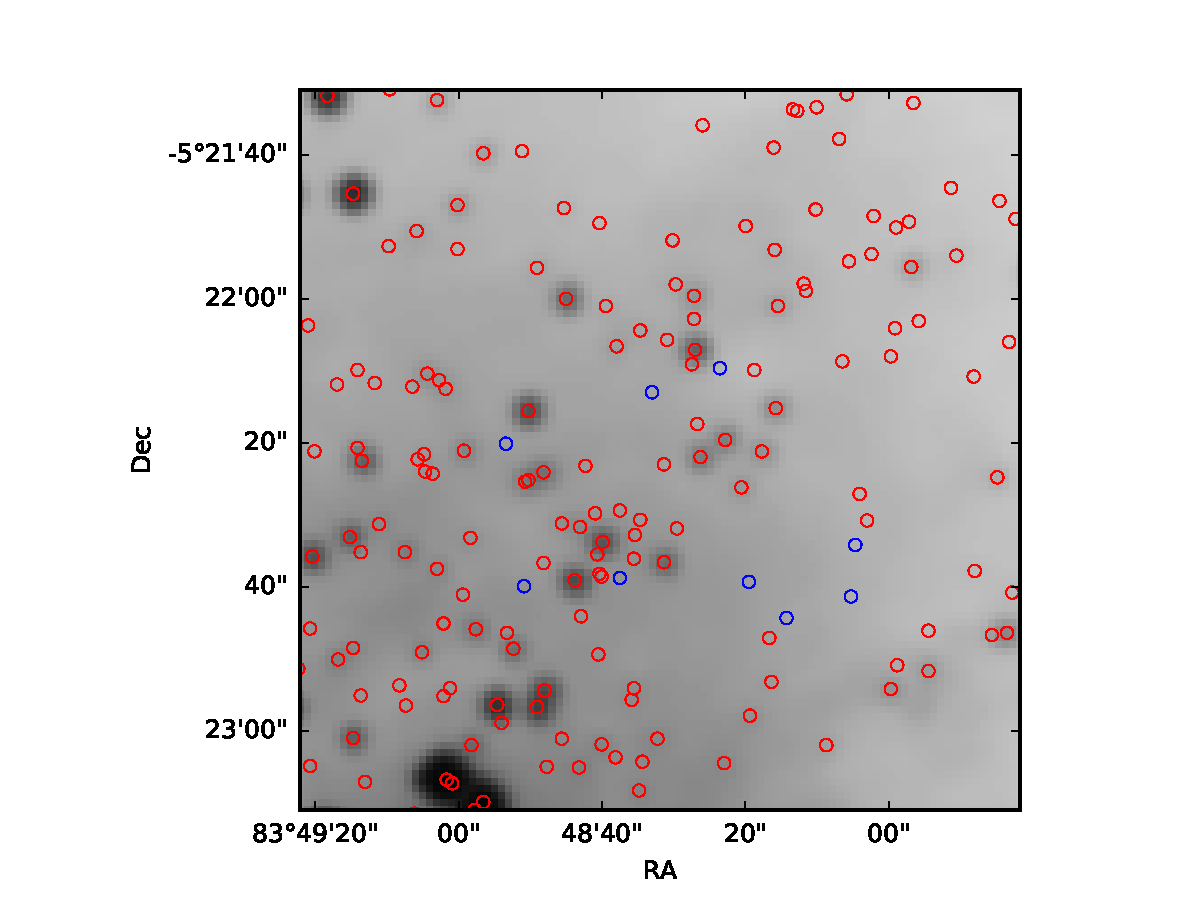
\includegraphics[scale=1,width=7in]{example_figure_1.pdf}
\caption{An example figure made using \astroquery's \texttt{skyview} and
\texttt{vizier} modules with \astropypkg's \texttt{table}, \texttt{coordinates},
\texttt{units}, and \texttt{wcs} modules.  The blue stars show sources from
an older, less complete catalog and the red circles show sources from a more
recent, more complete catalog.
}
\label{fig:example1}
\end{figure*}

\end{document}
